
\documentclass[12pt]{article}
\usepackage{graphicx}
\usepackage{hyperref}
\usepackage{amsmath}


\begin{document}

\begin{center}
\textbf{ MAT 442: HMW 4}\\
\textbf{\ Joseph Mensah (Spring 2019)}\\
\end{center}

\begin{enumerate} 
\item Example 3 on page 7, we check the stability of the 2 cycle for the \textbf{Ricker model}: For $a=9$ , $b=5$ and \[y_{k+1}=ay_ke^{by_k},  \hspace{0.5cm}a>1\]
Using the cobweb method we obtain

\begin{figure} [ht!]
 \centering
 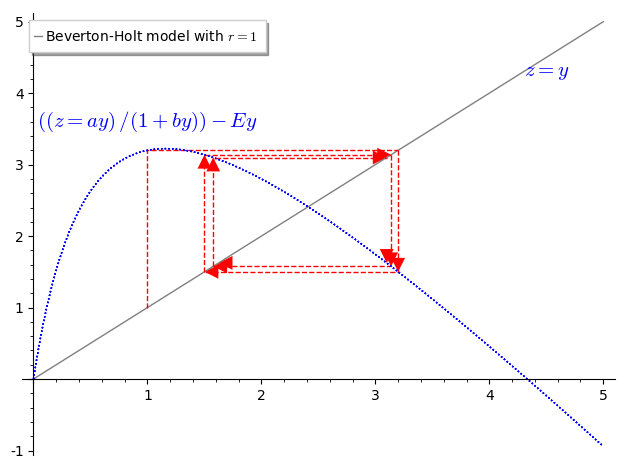
\includegraphics[height=4in]{/Users/ERICAGYEMANG/Desktop/Biomath/Figures/tmp4.jpg} 
\caption[Figure 2.4: r>1]{The cobweb diagram shows an oscillating movement around the equilibrium this means it is not approaching zero or extinction.}
 \label{fig::model}
\end{figure}


(b) we compute positive equilibrium point and check the stability
\begin{align*}
&f(y)=\frac{ay}{1+by}-Ey=y\\
&\Rightarrow by^2+Eby^2+y+Ey-ay=0\\
&\Rightarrow y(by+Eby+1+E-a)=0\\
&\Rightarrow by+Eby=1-E-a\\
&\Rightarrow y(b+E)=\frac{a-E-1}{b+E}\\
&\Rightarrow y=\frac{1}{b}(\frac{a}{E+1}-1)\\
\mbox{thus}\\
&\boxed{y_\infty=(\frac{a}{E+1}-1)/b}.\\
\end{align*}

Now we find the derivative and substitute $y_\infty$,we have 

\begin{align*}
f'(y_\infty)=&\frac{a}{[1+b(\frac{1}{b}(\frac{a}{E+1}-1))]^2}-E\\
=&\frac{a}{(\frac{a}{E+1})^2}-E\\
=&\frac{(E+1)^2}{a}-E>0(\mbox{we assume}\hspace{0.1cm} E>0).\\
\end{align*}
For the nonzero equilibrium to be LAS, we want\\

$-1<\frac{(E+1)^2}{a}-E<1\Leftrightarrow E-1<\frac{(E+1)^2}{a}<E+1\Leftrightarrow \boxed{\frac{E-1}{E+1}<\frac{E+1}{a}<1}$,
the RHS of the inequality is satisfied because algebraic manipulation on RHS will give us \boxed{\frac{E+1}{a}<1\Leftrightarrow E<a-1} \hspace{0.1cm}\mbox{hence}\hspace{0.1cm} $E<A-1$ is satisfied.For LHS of the inequality we have \boxed{\frac{E-1}{E+1}<\frac{E+1}{a}\Leftrightarrow a<\frac{(E+1)^2}{E-1}} which automatically satisfies the condition because if $E<1$ then $\frac{E-1}{E+1}<0$ so either one gives us LAS for the positive equilibrium.\\

(c) In this part we derive the opposite conclusion to part(b) when the parameters do not give rise to LAS condition. 
For the first part we check what happens(behavior) using cobweb graph(Figure 1) when $a>\frac{(E+1)^2}{E-1}$.\\

For the second part we check what happens when\hspace{0.1cm} $a<E-1$\hspace{0.1cm}.It is obvious there is a contradiction because in part (a) above it was established that zero equilibrium is LAS when $E-1<a<E+1$.There is zero equilibrium which is unstable hence population move towards extinction.

\begin{figure} [ht!]
 \centering
 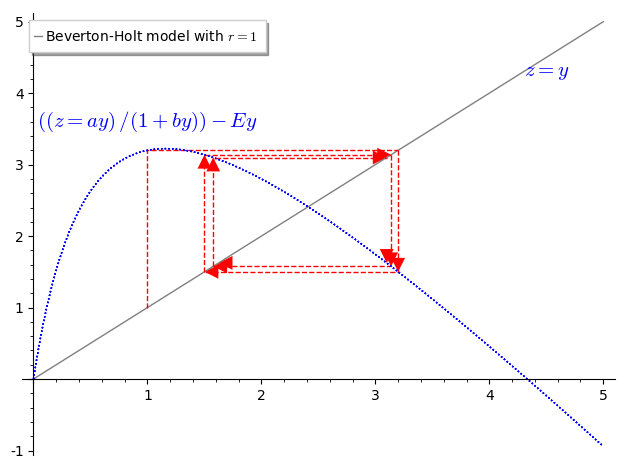
\includegraphics[height=4in]{/Users/ERICAGYEMANG/Desktop/Biomath/Figures/tmp4.jpg} 
\caption[Figure 2.4: r>1]{The cobweb diagram shows an oscillating movement around the equilibrium this means it is not approaching zero or extinction.}
 \label{fig::model}
\end{figure}

\cleardoublepage 

\item Comparing the existence and stability of equilibrium points, as well as the general characteristics of solutions of Beverton-Holt model.

\textbf {(a) no harvesting}\\
The equilibrium points are $y_\infty^1=0$ if $a<1$(make it is stable) and $y_\infty^2=(\frac{a-1}{b}$ if $a>1$(makes it unstable).\\

\textbf {(b) constant-rate harvesting}\\
The equilibrium points are \[y_\infty=\frac{1}{2}[(\frac{a-1}{b}-H)\pm \sqrt{(\frac{a-1}{b}-H)^2 -4\frac{H}{b}}\].\\

\textbf {(c) constant-effort harvesting}\\
The equilibrium points are $y=0$ and $y_\infty=(\frac{a}{E+1}-1)/b$.For the nonzero equilibrium to be LAS, we want

$-1<\frac{(E+1)^2}{a}-E<1\Leftrightarrow E-1<\frac{(E+1)^2}{a}<E+1\Leftrightarrow \boxed{\frac{E-1}{E+1}<\frac{E+1}{a}<1}.$\\

\textbf {Conclusion:} In \textbf {no harvesting} which has two outcomes either $y=0$  if $a<1$ for stability where there is no need to introduce harvesting because fish population  will move towards extinction or zero equilibrium.The other case for \textbf {no harvesting} is unstable if $a>1$ which is pretty useful because there is excessive(rapid) growth of fish population.For \textbf{constant-rate harvest} it was established that to promote better modeling  techniques for fish population can withstand harvesting without the fish population going to extinction and for what rate of harvesting will there be a positive asymptotically stable equilibrium.In \textbf{constant-effort harvesting} there is an exerted Effort "E" and constant yield $Ey$.Since Beverton Holt model is a typical example for contest competition, some effects of harvesting in contest competition can lead to extinction of species and also harvesting occurring in finite time space.When harvesting is introduced to Beverton model it can lead to jump in equilibrium called catastrophe, meaning the fish population will be wipe out as a result of harvesting rate $H$ increasing beyond certain value of threshold where there is no equilibrium.(Figure 2.21-2.23 on p.63 of our textbook give a clear graph of the qualitative behavior). 

\cleardoublepage 



\item Section 2.5 Exercise 10 (p.68). Logistic model with constant-effort harvesting.\\
(a) \[\boxed{f(y)=ry(1-\frac{y}{k})-Ey.}\]
To find equilibrium points, set
\begin{align*}
&f(y)=ry(1-\frac{y}{k})-Ey=y\\
&\Rightarrow ry-\frac{ry^2}{k}-Ey-y=0\\
&\Rightarrow y(\frac{-ry}{k}+(r-E-1))=0\\
&\Rightarrow\frac{-ry}{k}=-r+E+1\\
&\Rightarrow y=\frac{k}{r}(r-E-1)\\
&\Rightarrow y=k(1-\frac{E}{r}-\frac{1}{r})\\
\end{align*}



(b) we have the equilibrium points to be
\[\boxed{y_\infty^1=0\hspace{0.2cm} \mbox{and} \hspace{0.2cm}y_\infty^2=k(1-\frac{E}{r}-\frac{1}{r}).}\]
Now for all the non negative equilibrium points, with conditions on the parameters for the positive equilibrium we want
\begin{align*}
y_\infty^2=k(1-\frac{E}{r}-\frac{1}{r})&>0\\
       1-\frac{E}{r}-\frac{1}{r}&>0\\
       r-E-1&>0\\
       E&<r-1.
\end{align*}

(c) To study the stability of nonnegative equilibria analytically we find the derivative of $f$ ,substitute $y_\infty^1\hspace{0.1cm} \mbox{and}\hspace{0.1cm} y_\infty^2$ to obtain
\[f'(y)=r-y-2y-E\Rightarrow f'(y_\infty^1=0)=\boxed{r-E}.\]
For the stability of zero equilibrium: We set\\
\[-1<r-E<1\Leftrightarrow r-1<E<r+1\] 


For the stability of positive equilibrium: we have
\[f'(y_\infty^2)=r-\frac{2r}{k}(k(1-\frac{E}{r}-\frac{1}{r})-E=r-2r+2E+2-E=\boxed{E-r+2}.\]
For the equilibrium to be LAS, we need
\[-1<E-r+2<1\Leftrightarrow -3<E-r-1\Leftrightarrow r-3<E<r-1.\]


\cleardoublepage

\item Comparing the existence and stability of equilibrium points, as well as the general characteristics of solutions of Logistic model.

\textbf {(a) no harvesting}\\
The equilibrium points are $y_\infty=0$ and $y_\infty=k(1-\frac{1}{r})$, as per our LN 3 we established that $\left|f'(0)\right|=r>1$,so that 0  is always unstable and $\left|2-r\right|<1\Leftrightarrow -1<r-2<1\Leftrightarrow 1<r<3.$



\textbf {(b) constant-rate harvesting}\\
The equilibrium points are 
 \[y_\infty=\frac{1}{2}(k(1-\frac{1}{r})\pm \sqrt {k^2(1-\frac{1}{r})^2 -4\frac{Hk}{r}})\],from our LN5 we know that \[f'(y_-)=1-\sqrt{(r-1)^2-\frac{4rH}{k}}\] therefore, there is an existence of stability.
 

\textbf {(c) constant-effort harvesting}\\
The equilibrium points are $y_\infty^2=0$ and $y_\infty^2=k(1-\frac{E}{r}-\frac{1}{r})$.For the stability of zero equilibrium we set $-1<r-E<1\Leftrightarrow r-1<E<r+1$ and for stability of positive for the LAS we need, $-1<E-r+2<1\Leftrightarrow r-3<E<r-1$. \\

\textbf{Conclusion:}
In \textbf{no harvesting} for logistic model with $r>>1$ there will be no asymptotically stable equilibrium.For \textbf{constant-rate harvesting} in logistic model there is upper bound interval($H_{max}$) and lower bound interval($H_{min}$)  when $r>3$ we can derive means of stability by regulating the population through harvesting this avoids fluctuations in the fish population and keeps it steady.From the previous Homework we know that scramble competition with discrete logistic growth model and fertility growth rate $r>>3$ has no LAS  positive equilibrium meaning there is higher movement in chaotic manner so introducing harvesting into this population will regulate the population rise, keep it in a steady manner so there will be enough resources for fish to also feed on.When $Ey$ thus \textbf{constant-effort harvesting} is applied to the discrete model there will be more fish to catch because default logistic model with no harvesting has high fertility growth rate $r>>3$ in scramble competition.






\end{enumerate}

\cleardoublepage

\begin{thebibliography}{99}
\bibitem{r1}Dynamical Systems for Biological Modeling: An Introduction by Brauer and Kribs, CRC Press, 2016. ISBN 978-1-4200-6641-8


\end{thebibliography}

\end{document}